

\subsection{Databases}

\textbf{JB to compile descriptions?}

\subsection{Antineutrino Detector Data}

Photomultiplier (PMT) data from the PROSPECT Antineutrino Detector (AD) is acquired as waveforms using CAEN V1725 Waveform Digitizers (WFDs).
Firmware on the WFDs forms a coincidence trigger between the two PMTs attached a segment. 
When any one segment triggers, a NIM pusle is distributed to every WFD module to initiate acquisition of waveforms for every PMT. 
148 samples of data, spaced by 4 ns, are acquired for each channel.
Firmware on the WFD then performs zero-length-encoding (ZLE) to suppress readout of baseline data on PMTs where there is no particle interaction signal.
If the initial 150 sample waveform contains signals above a ZLE threshold, between 56 and 148 samples are kept; otherwise, the waveform data is discarded.
In this way, data can be efficiently collected from the multi-segment detector without the need for a very low energy threshold (and consequently very high singles data rate) on each individual segment.

A total of 21 WFD modules are distributed between 8 CAEN CONET2 fiber-optic links, with 2 or 3 daisy-chained on each link.
Each WFD can buffer up to 1023 trigger events' data between (and continuing during) readouts.
Two CAEN A3818 controller boards with 4 links per boards are used separately in two DAQ control computers.  
Each optical link is controlled and read out through a dedicated process, which cycles through reading out its WFDs' buffers.
These 8 ``DAQDumper'' processes record the data streamed over the optical link from each WFD module to the network-mounted local storage array ``blue.''
Therefore, the initial form of the detector data recorded to disk is 8 separate binary files per run.
The data contained within these files and subsequent processing are described in Sec.~\ref{sec:processing}.
During the run, an additional copy of the data is streamed over the local network to produce real-time plots displayed on a monitoring webpage.
The live data streaming is separate from the process writing to disk, and may be interrupted or stopped with no impact on DAQ operation.
Run metadata, such as the start time and acquisition thresholds, is recorded to a DAQ database when the run is started.
After run completion, additional metadata including the run time, file size, and md5 checksum for the raw data is entered into the DAQ database.

The raw data production rate varies considerably with the running mode of the PROSPECT AD and the status of the HFIR reactor.
Typical data rates for various conditions are given in Table~\ref{tab:dataRates}. 

\begin{table*}[tbp]
  \begin{centering}
  \begin{tabular}{l|lll}
  Quantity/Run Condition& Reactor On & Reactor Off & Calibration \\ \hline
  Acquisition Event Rate (kHz) & 40 & 5 &  25 \\
  Segment Event Rate (kHz) & 160 & 35 &  140 \\
  Avg. Segment Multiplicity & 4.0 & 7.0 &  5.X \\
  Max Opt. Link Rate (MB/s) & 8.0 & 1.0 &  XXX \\
  Min Opt. Link Rate (MB/s) & 4.0 & 0.6 &  XXX \\
  Data Transfer Rate (MB/s) & 25 & XXX &  XXX \\
  Data Volume per Run (MB/s) & XXX & XXX &  XXX \\
  Data Volume per Day (GB) & XXX & XXX &  XXX \\
  \end{tabular}
  \caption[dataRates]
  {Data acquisition and transfer parameters for three typical operating conditions. Number needs to be checked. Define run length.
  Define calibration condition here.
  Avg multiplicity is higher for reactor off because muon and other cosmic events have very high multiplicity; these are are greater fraction of events with the reactor off(RxOFF)}
  \label{tab:dataRates}
  \end{centering}
\end{table*}

\rvnote{Is there any local data analysis for quality monitoring?}
% MM: yes, CrunchLive system runs a live analysis with plots output to a webpage for quality monitoring

\begin{figure}
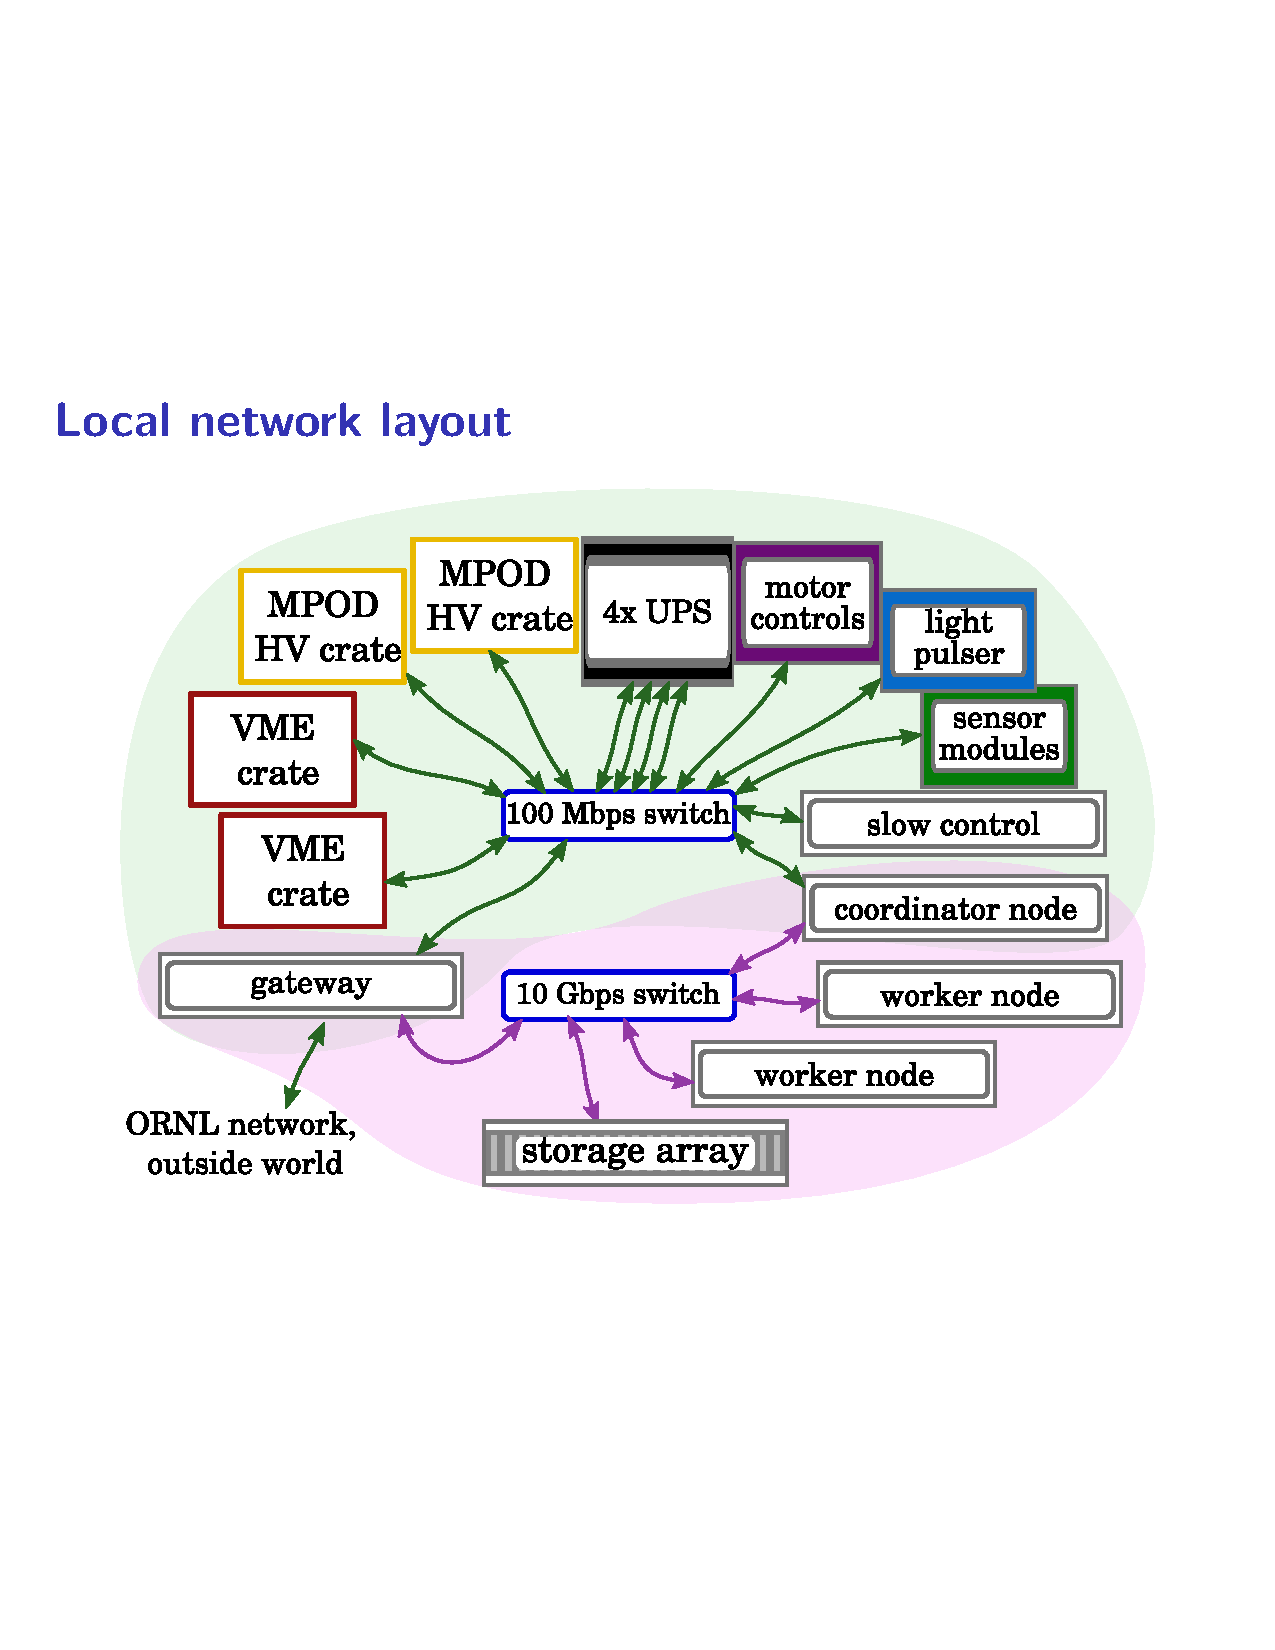
\includegraphics[width=0.75\textwidth]{figures/DAQ_NetworkPlan.pdf}
\caption{Network connectivity of the detector DAQ} \label{fg:daqnet}
\end{figure}

The detector local data acquisition network architecture is shown in Fig~\ref{fg:daqnet}.
The storage server, DAQ control computers, and data transfer gateway server are connected
	by a high-speed 10\,Gb/s ethernet local network.
A separate 100\,Mb/s local network is used for controlling DAQ rack components (power supplies and VME crates),
	and ``slow control'' environmental sensors and calibration system components.

The data are transfered to long term storage and processing at LLNL.
This process is driven by Python scripts that consult the DAQ database for status and determines the current step of the data transfer.
Pull requests by oslic.llnl.gov are made every 31 minutes to move data off of the storage array.
The network connection from the gateway to the Internet is 1\,Gb/s, limited by the HFIR network infrastructure.  
